\documentclass[11pt,a4paper]{article}

% Page geometry
\usepackage{geometry}
\geometry{left=2.54cm,
	right=2.54cm,
	top=2.54cm,
	bottom=2.54cm}
\parskip 0.15cm
\setlength{\parindent}{0cm}

% Font
\usepackage{lmodern}
\usepackage[T1]{fontenc}

% English language
\usepackage[utf8]{inputenc}
\usepackage[UKenglish]{babel}
\usepackage{csquotes}

% Images 
\usepackage{graphicx}  % Extended image support
\usepackage{float}  %  Graphics placement [H] [H!] arguments
\usepackage{caption}  % Custom captions
\usepackage{subcaption}  % Compound figures

\makeatletter
	\g@addto@macro\@floatboxreset\centering  % Automatically centre images (floats)
\makeatother

% Tables
\usepackage{booktabs}  % Sensible horizontal rules
\usepackage{array}  % Extended column formats
\usepackage{multirow}  % Tables with cells split over multiple rows
\usepackage{longtable}  % Tables spanning multiple pages
\usepackage{makecell}  % Multi-row table headers
\renewcommand\theadfont{}  % Don't reduce font size of \thead

% Bibliography 
\usepackage[natbib, 
	style=authoryear, 
	uniquename=false, 
	uniquelist=false,
	giveninits=true,
	dashed=false,
	maxcitenames=2, 
	mincitenames=1, 
	minbibnames=10, 
	maxbibnames=10, 
	sortcites,
	backend=biber]{biblatex}
\renewcommand*\finalnamedelim{\addspace\&\space}

% Text formatting
\usepackage{enumerate}  % Enumerated lists
\usepackage{lineno}  % Line numbers
\usepackage[group-separator={,}]{siunitx}  % Units
\usepackage{amsmath}  % Math symbols
\usepackage{amssymb}  % Math symbols
\usepackage[table]{xcolor}  % text colours
\newcommand{\todo}[1]{\textcolor{red}{\textbf{#1}}}   % \todo{NOTE IN RED}
\usepackage{framed}  % Framed boxes
\usepackage{microtype}  % Improved text justification
\usepackage{listings}  % Code input 
\renewcommand{\lstlistingname}{Code}  % Rename code chunks
\definecolor{menu}{RGB}{0,102,204}
\newcommand\menu[1]{\texttt{\color{menu}#1}}  % define in-line code formatting
\definecolor{file}{RGB}{0,153,76}
\newcommand\file[1]{\texttt{\color{file}#1}}  % define in-line code formatting
\definecolor{numval}{RGB}{204,102,0}
\newcommand\numval[1]{\texttt{\color{numval}#1}}  % define in-line code formatting

% Define code colours
\definecolor{codegreen}{RGB}{16,154,39}
\definecolor{codegray}{RGB}{92,92,92}
\definecolor{codepurple}{RGB}{131,46,156}
\definecolor{backcolour}{RGB}{243,243,243}
\definecolor{bordercolour}{RGB}{0,0,0}

% Define code chunk aesthetics
\lstdefinestyle{mystyle}{
    backgroundcolor=\color{backcolour},
    commentstyle=\color{codegreen},
    keywordstyle=\color{magenta},
    numberstyle=\tiny\color{codegray},
    stringstyle=\color{codepurple},
    basicstyle=\ttfamily\footnotesize,
    breakatwhitespace=false,
    breaklines=true,
    captionpos=b,
    keepspaces=true,
    numbers=left,
    numbersep=8pt,
    firstnumber=1,
    showspaces=false,
    showstringspaces=false,
    showtabs=false,
    tabsize=2,
    frame=top,
    frame=bottom,
	framexleftmargin=5pt,
    rulecolor=\color{bordercolour}
}
\lstset{style=mystyle}

\lstdefinelanguage{json}{
    string=[s]{"}{"},
    comment=[l]{:\ "},
    morecomment=[l]{:"},
    literate=
        *{0}{{{\color{codepurple}0}}}{1}
         {1}{{{\color{codepurple}1}}}{1}
         {2}{{{\color{codepurple}2}}}{1}
         {3}{{{\color{codepurple}3}}}{1}
         {4}{{{\color{codepurple}4}}}{1}
         {5}{{{\color{codepurple}5}}}{1}
         {6}{{{\color{codepurple}6}}}{1}
         {7}{{{\color{codepurple}7}}}{1}
         {8}{{{\color{codepurple}8}}}{1}
         {9}{{{\color{codepurple}9}}}{1}
}

% Custom title formatting
\let\oldtitle\title
\renewcommand{\title}[1]{\oldtitle{\vspace{-1.5cm}#1}}

\usepackage{etoolbox}
\ifundef{\abstract}{}{\patchcmd{\abstract}%
    {\quotation}{\quotation\noindent\ignorespaces}{}{}}

% Links
\usepackage[breaklinks, hidelinks]{hyperref}
\definecolor{links}{RGB}{191,59,72}
\hypersetup{
	breaklinks,
	allcolors=links,
	linktoc=section,
	pdfauthor={John L. Godlee}
}

% Rename autorefs to capitals
\addto\extrasUKenglish{
        \renewcommand{\chapterautorefname}{Chapter}%
        \renewcommand{\sectionautorefname}{Section}%
        \renewcommand{\subsectionautorefname}{Section}%
        \renewcommand{\subsubsectionautorefname}{Section}%
}

\graphicspath{ {img/} }  % Define image path

\addbibresource{canopy_photo.bib}

\title{Photographic methods for measuring forest canopy structure}
\date{\today}
\author{John L. Godlee}

\begin{document}

\maketitle

\tableofcontents
\newpage

\section{Introduction}

This document is a set of curated notes on using photographic methods to measure forest canopy structure. Much of the document has been informed by personal experience in the field, and is supported by references found throughout the forestry and ecology literature. 

Canopy structure is highly variable within forests, being determined by species composition, abiotic environment, disturbance regime etc \citep{Fotis2018}. Canopy structure also has a large effect on ecosystem processes in forests. Leaf area is correlated with gross primary productivity of trees \citep{Chen2012}. Tree canopies determine the light environment and micro-climate below the tree canopy, with consequences for understorey biodiversity and community composition \citep{Bartels2010, Barbier2008}. Measuring forest canopy structure is therefore of interest to foresters, community ecologists, conservation scientists, and others.

There are myriad measures of canopy structure, each designed with a specific goal in mind. Forest canopies are a complex and multi-dimensional system. It is impossible to quantify every facet of canopy structure with a single method. Care must be taken to understand what the chosen measure of canopy structure is actually measuring, and whether this aligns with the needs of the research question.

\section{Common terms}

\begin{itemize}
	\item{Gap fraction - Proportional coverage of plant canopy material as viewed from a single point with some given angular field of view. Also known as the site factor or canopy closure \citep{Anderson1964}.}
	\item{Canopy cover - Proportional coverage of plant canopy material per unit ground area covered.}
	\item{Leaf/Plant Area Index (LAI/PAI) - Area of leaf (LAI) or plant (PAI) per unit ground area, most often expressed in m\textsuperscript{2} m\textsuperscript{-2}. LAI/PAI can be greater than 1 if plant material overlaps. PAI includes non-leaf plant material like stems.}
\end{itemize}

\begin{figure}[H]
\centering
	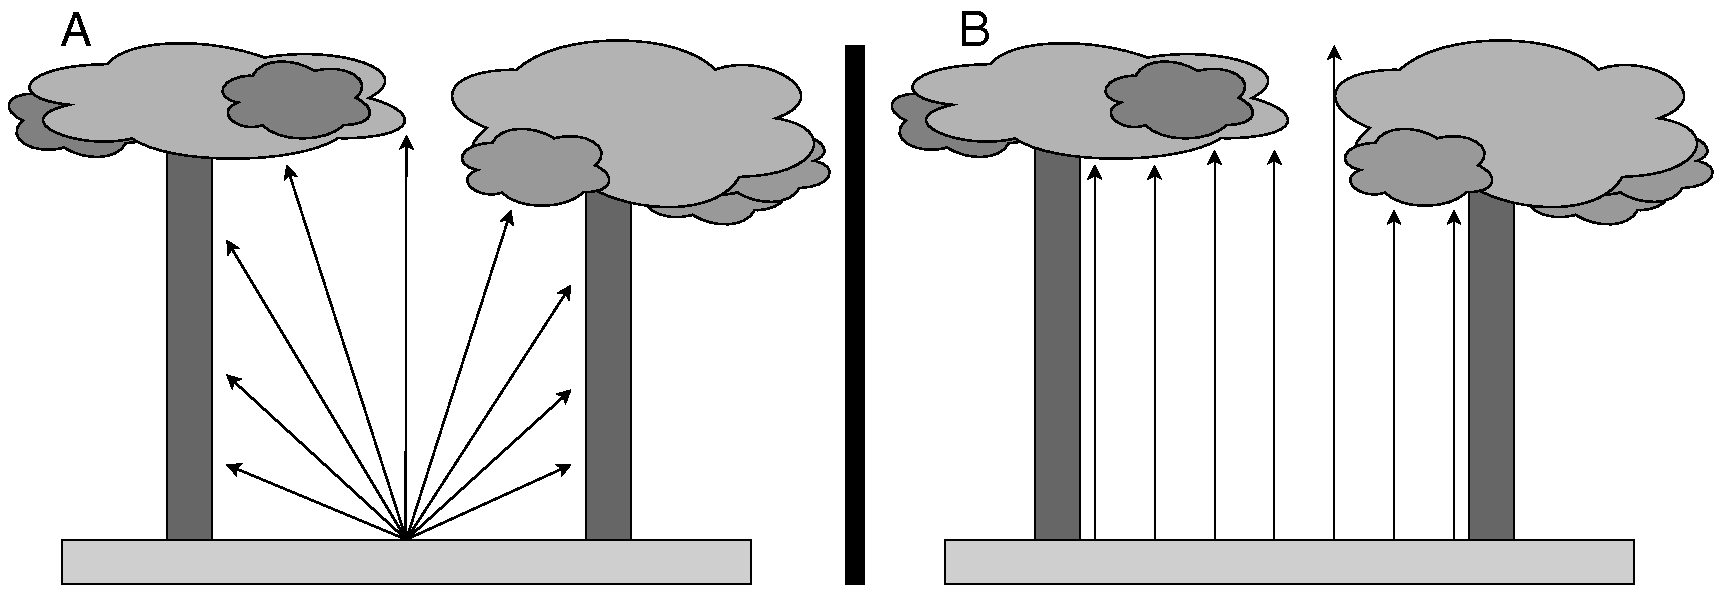
\includegraphics[width=\textwidth]{closure.drawio.pdf}
	\caption{Gap fraction (left) measured from a single point with a given angular field of view, compared with canopy cover (right) measured as the vertical projection of tree material onto the ground (Adapted from \citealt{Jennings1999}).}
	\label{closure}
\end{figure}

\section{Hemispherical photography}

Hemispherical photography is a technique where forest canopy structure is measured from photographs taken using a wide-angle fisheye camera lens. \citep{Seidel2011, Macfarlane2014}. 

\begin{figure}[H]
\centering
	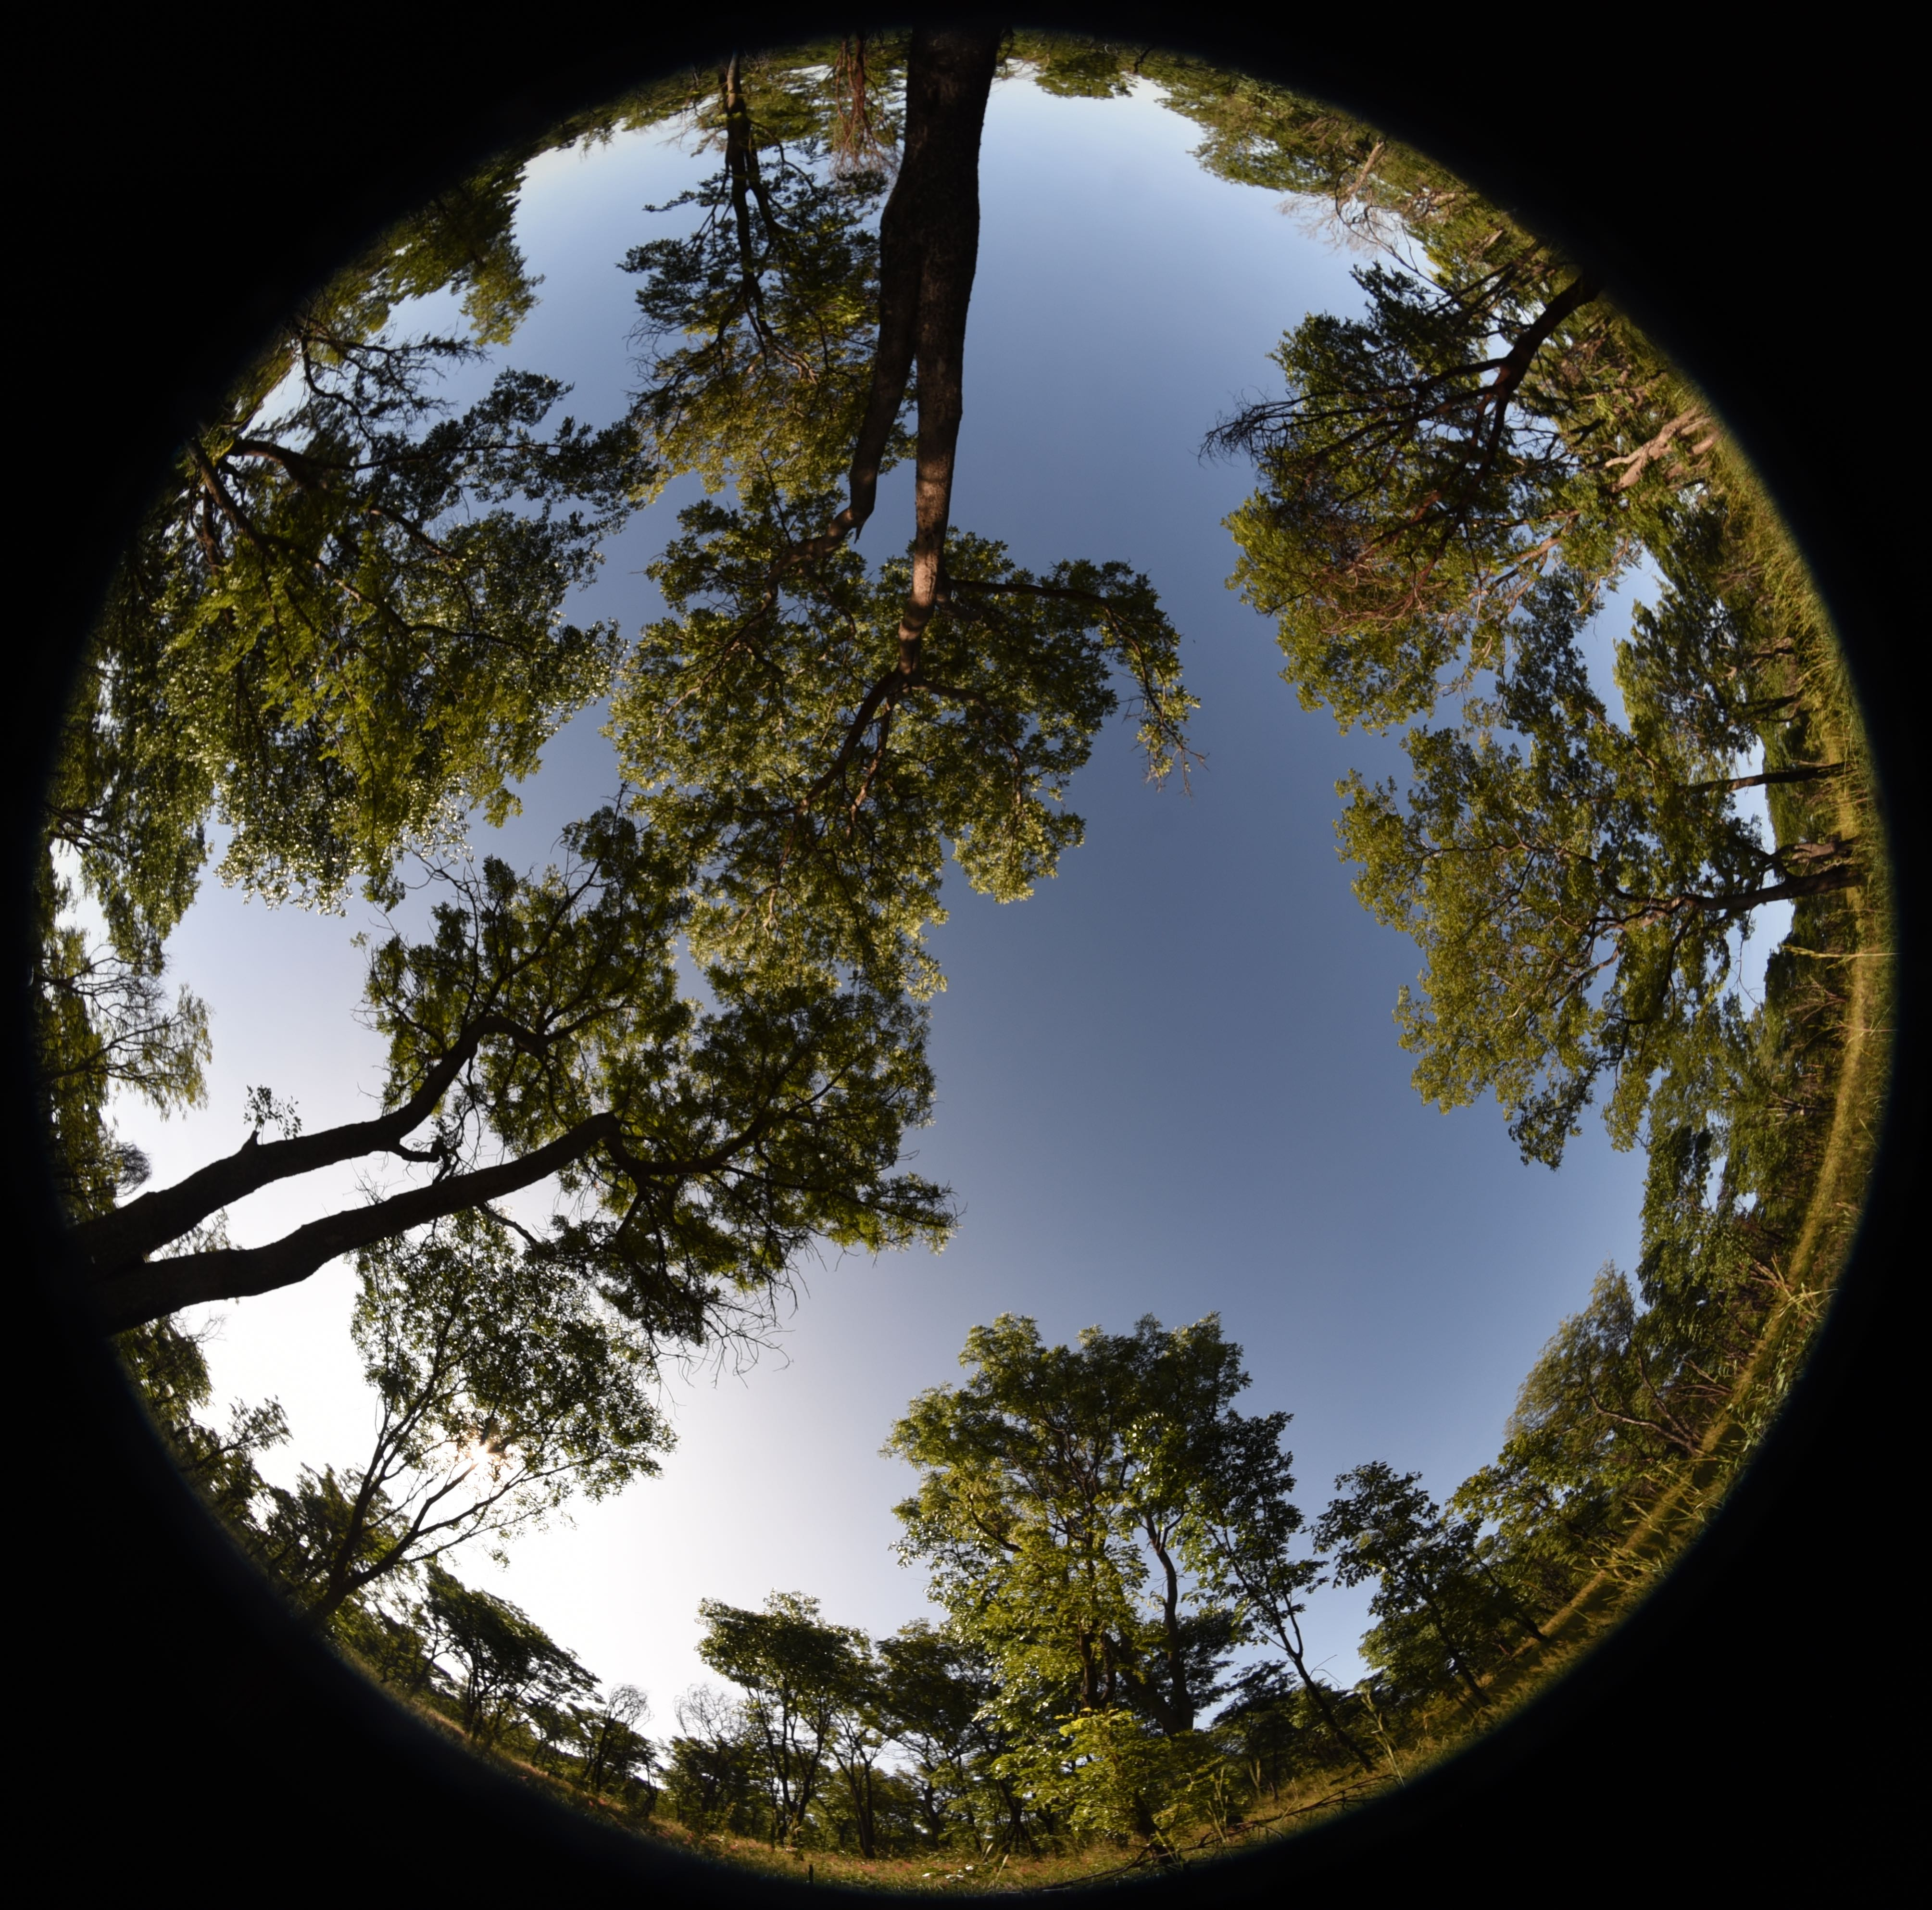
\includegraphics[width=0.5\textwidth]{hemi.jpg}
	\caption{An example of a hemispherical photo of a miombo woodland canopy in Bicuar National Park, southwest Angola.}
	\label{hemi}
\end{figure}

Hemispherical photographs can be analysed in multiple ways to provide different metrics of canopy structure. All these metrics are related and rely fundamentally on the classification of pixels in the photo into either plant material or sky. Different metrics are used depending on the convention of the field of research and according to the research question being asked. 

\subsection{Capturing informative hemispherical photos} \label{inform}

Taking digital hemispherical photos under field conditions which are representative of the forest canopy requires careful balancing of camera settings. Alas, there is no convention or consensus on acquisition of hemispherical images or their analysis \citep{Beckschafer2013}. Measurements of gap fraction from hemispherical photographs are sensitive to camera exposure \citep{Macfarlane2000}, image processing \citep{Jonckheere2004}, and gamma correction \citep{Macfarlane2007a}. 

Confident use of the many settings available on a modern DSLR camera is necessary to adjust for environmental conditions which may change throughout the day to gather consistent and informative images. Some common issues which create bias in results:

\begin{itemize}
	\item{Lens flare - Bright sunlight reflects within the lens due to material imperfections in the lens glass, causing haze and starburst artefacts in the image (\autoref{lens_flare}).}
	\item{Blooming - An over-saturated part of the image ``bleeds'' into other pixels on the image sensor during image capture. This is the most common problem in hemispherical photography and is highly sensitive to image exposure.}
	\item{Obstructions between camera and canopy - Understorey vegetation, man-made objects, the head of the camera operator.}
\end{itemize}

\begin{figure}[H]
\centering
	\includegraphics[width=0.6\textwidth]{lens_flare}
	\caption{An example of a hemispherical photo with excessive lens flare. In this example, gap fraction will appear higher than in reality, as the bright lens flare will be classified as sky unless extra processing is applied to the image.}
	\label{lens_flare}
\end{figure}

There is no standard protocol for hemispherical photography. Capturing an informative image relies on manual adjustment of three key camera settings to balance the image exposure and sharpness:

\begin{itemize}
	\item{Shutter speed - the length of time the shutter is open while the
		image is being captured}
	\item{Lens aperture - the size of the hole through which light enters 
		the camera lens}
	\item{ISO - analogous to the sensitivity of the sensor to incoming light}
\end{itemize}

Below is a guide to taking good hemispherical photographs: 

\begin{itemize}
	\item{Take photos under a uniformly overcast sky where possible, ideally before the sun has risen high in the sky, or just before sunset. This avoids lens flare and increases contrast between plant and sky. In the morning the photos are generally better due to the quality of the light and the generally more consistent cloud cover. At high latitudes there is a longer suitable period to capture photos than in the tropics where sunrise and sunset are quick.}
	\item{Ensure that the camera is level on a tripod and the lens is pointing straight up towards zenith. Use a spirit level attached to the camera hotshoe to level the camera.}
	\item{Adjust the tripod so that the top of the camera lens is 1.3 m above the ground, or above any understorey vegetation, which is not considered part of the canopy, whichever is higher.} 
	\item{Turn the camera so the top of the camera body is facing north. This ensures that the top of the captured photo is also facing north. Some measures of canopy structure rely on knowing the path of the sun across the image.}
	\item{Make use of the camera's screen display, if there is one, to inspect the field of view before capturing the photo.}
	\item{Set the camera. Note that these settings work for my camera, listed in the  
		``ideal list of products'' below, and are subjective:}
		\begin{itemize}
			\item{Manual shooting mode}
			\item{Manual focus}
			\item{Set the focus to infinity}
			\item{Set the exposure compensation to -0.7 \citep{Zhang2005}}
			\item{Capture fine \file{.jpg} and RAW images at the same time}
			\item{Ensure the camera time and date is accurate, for ease of matching photos to sites during analysis}
			\item{Set the Aperture to \textasciitilde{}f7-9. We don't want pretty bokeh, just crisp images.}
			\item{Adjust the ISO and shutter speed so the photo is neutrally exposed but the shutter speed is always over 1/100sec, slow shutter speeds introduce camera shake. If it is windy check the photos for blurry tree branches and adjust the shutter speed accordingly.}
			\item{If the camera attempts to intelligently rotate photos based on the camera orientation, disable this feature and make sure all photos are captured in landscape orientation.}
		\end{itemize}
	\item{Make sure everybody ducks down below the camera when the image is taken!}
	\item{Cover the lens with the lens cap between photos to prevent scratches on the lens.}
\end{itemize}

A daily kit list for taking hemispherical photos:

\begin{itemize}
	\item{Camera with appropriate fisheye lens}
	\item{Lens cap}
	\item{Lens cleaning solution and lens cloth}
	\item{Tripod}
	\item{At least 2 fully charged batteries for camera}
	\item{2 SD cards}
	\item{Spirit level hotshoe attachment for camera}
	\item{Compass}
	\item{Notebook and pencil}
	\item{Handheld GPS unit}
	\item{Tape measure >2 m}
	\item{Waterproof bag to cover camera}
\end{itemize}

An ideal list of products for a high quality DSLR camera setup:

\begin{itemize}
	\item{Nikon D750 DSLR camera body}
	\item{Sigma 8 mm f3.5 circular fisheye EX DG for Nikon lens}
	\item{Generic hotshoe spirit level}
	\item{Integral USB SD card reader}
	\item{2x Sandisk Ultra 30 MB/s SDHC card 16 GB Class 10}
	\item{Hard peli-case to fit equipment in, e.g. Peli-1520 with foam}
	\item{A sturdy tripod}
\end{itemize}

Note that the tripod needs to be able to tilt the camera so the lens points straight up. This is difficult with many tripods. Alternatively, add a gimbal which attaches to the top of the tripod. Adding a gimbal is often cheaper than buying a new tripod.

\subsection{Sampling strategy}

In order to estimate the mean value of various metrics of forest canopy structure over an area of forest, multiple photos must normally be taken. Determining the spatial distribution of these photos is therefore necessary to ensure that a representative sample of the forest canopy is achieved. The shape of the sampling area will somewhat determine the spatial pattern of photos, circular plots may require a different layout to rectangular plots and linear transects, for example.

During analysis it is common to restrict the field of view of the hemispherical photo to 60\textdegree{}. See \autoref{fov} for more information. With this in mind, a simple calculation with some sensible assumptions can estimate the minimum distance of photos to avoid pseudo-replication of the canopy area:

\begin{equation}
	D = 2D_{\theta} = 2(h \tan{\theta})
\end{equation}

where $\theta$ is the angular field of view in degrees, $h$ is the height from the camera lens to the base of the canopy, and $D$ is the minimum distance of photos to avoid pseudo-replication of canopy area.

\begin{figure}[H]
\centering
	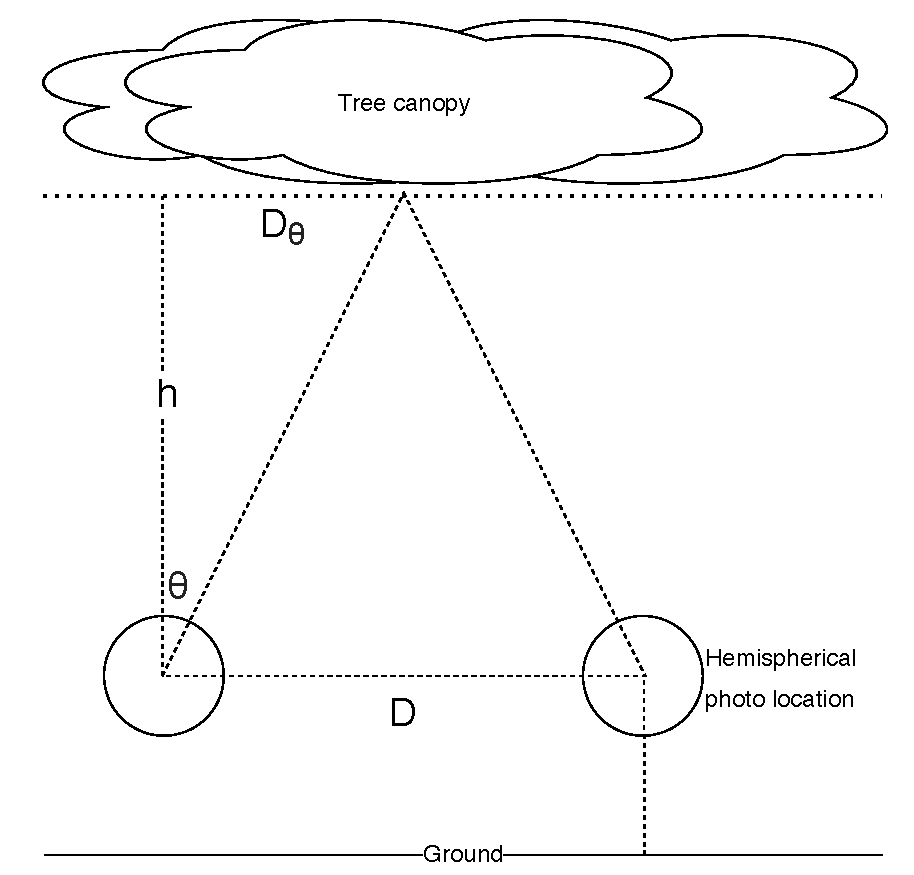
\includegraphics[width=0.5\textwidth]{canopy_trig.drawio}
	\caption{Schematic diagram of the measurements used when calculating the minimum distance between hemispherical photo locations.}
	\label{canopy_trig}
\end{figure}

In a square plot where the goal is to understand the mean and variance of canopy gap fraction, it is common to distribute photos in a grid over the plot (\autoref{hemi_layout}). It may also be necessary to place photo locations sufficiently inside the plot boundaries to avoid sampling areas of the canopy outside the plot. Again, the equation above can help with this calculation.

\begin{figure}[H]
\centering
	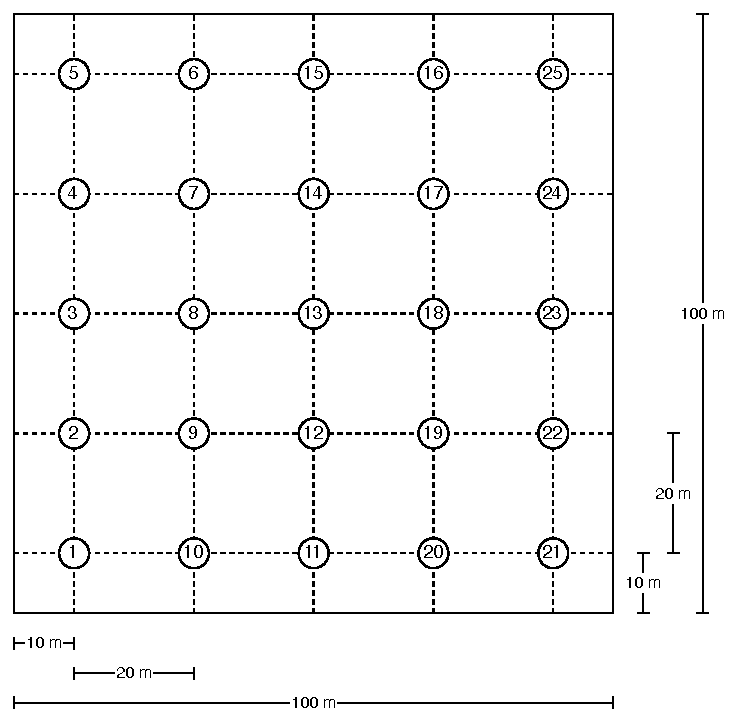
\includegraphics[width=0.5\textwidth]{hemi_layout.drawio}
	\caption{Diagram showing one possible layout for hemispherical photo locations within a 100x100 m square forest plot.}
	\label{hemi_layout}
\end{figure}

\subsection{Setting the focus to infinity} 

My assumption has always been that when taking hemispherical photos of forest canopies, the focus of the lens should be set to infinity. While this knowledge is repeated throughout the literature, it is difficult to find much discussion on \textit{why} this is the case. What follows is a series of quotes from the literature on the discussion of setting the lens focus to infinity.

\begin{minipage}{\linewidth}
\begin{framed}
We used a Nikon MF-16 camera and a Nikkor 8-mm fish-eye lens with TriX ASA 400 film, a red filter to increase sharpness of leaf edges, and the \textit{focus set to infinity}.

-- \citealt{Englund2000}
\end{framed}
\end{minipage}

\begin{minipage}{\linewidth}
\begin{framed}
The lens was set to a small aperture and \textit{focused on infinity} (Frazer et al. 2001; Zhu et al. 2003)

-- \citealt{Hu2009}
\end{framed}
\end{minipage}

\begin{minipage}{\linewidth}
\begin{framed}
Exposure settings were selected to obtain the best contrast between foliage and sky and making the last one appear white (cloudy sky offers the best condition in this context). The camera was used in automatic mode using the parameters fixed in FISHEYE1 lens mode (\textit{focus set to infinity}, widest zoom, metering center-weighted), and the shutter speed was varied automatically by the camera.

-- \citealt{Paletto2009}
\end{framed}
\end{minipage}

This next quote comes from a paper which many others reference when describing proper protocol for taking hemispherical photos: 

\begin{minipage}{\linewidth}
\begin{framed}
Unlike the Nikon F, the digital camera did not allow full manual control of both the shutter speed and lens aperture. We therefore \textit{set the autofocus, exposure mode, and f-stop of the digital camera to infinity}, aperture priority (shutter speed is set automatically by the camera), and f/2.6, respectively. 

-- \citealt{Frazer2001}
\end{framed}
\end{minipage}

While this next paper is one of the most respected guides on hemispherical photography, it references an unconventional source when describing the practice of setting the focus to infinity. A downloadable tutorial series on taking high-quality digital photos, called 123di \citep{123di}. Most of this resource is behind a pay-wall, so I can't read the applicable bit. Importantly however, this paper mentions \textit{why} the authors set the focus to infinity, because the depth of field is practically infinite under these conditions.

\begin{minipage}{\linewidth}
\begin{framed}
Photographic images were recorded using a Sigma 8 mm f/4 fisheye lens (Sigma Corporation, Tokyo, Japan) at the highest possible resolution (3040-2008 pixels) with highest ISO setting (ISO 200). Moreover, \textit{the focus ring was set to infinity when using the fisheye lens, as depth of field is practically infinite and focusing was not required (Bockaert, 2004).}

-- \citealt{Jonckheere2005}
\end{framed}
\end{minipage}

\section{Digital cover photography}

Measurements derived from hemispherical photography are highly sensitive to image acquisition and processing methods. Additionally, hemispherical photography equipment can be expensive.

Digital Cover Photography (DCP) uses flat images taken using a conventional camera lens. DCP was first used by \citet{Macfarlane2007a}. DCP has a higher sampling resolution closer to zenith, because the image is taken with a flat lens. This bias actually aligns somewhat with the importance of the canopy overhead for understorey light regime, and so isn't actually a big problem. DCP requires independent measurements of leaf inclination angle to estimate LAI \citep{Ryu2010}, but can be more appropriate for estimating canopy cover in certain circumstances \citep{Pekin2009}. Gap fraction cannot be measured directly with DCP because gap fraction needs the full hemisphere, but it can be modelled using allometric equations if necessary.

As a flat lens image will have a restricted field of view compared to a hemispherical photo, it may be necessary to increase sampling density within the area of forest of interest. 

\begin{figure}[H]
	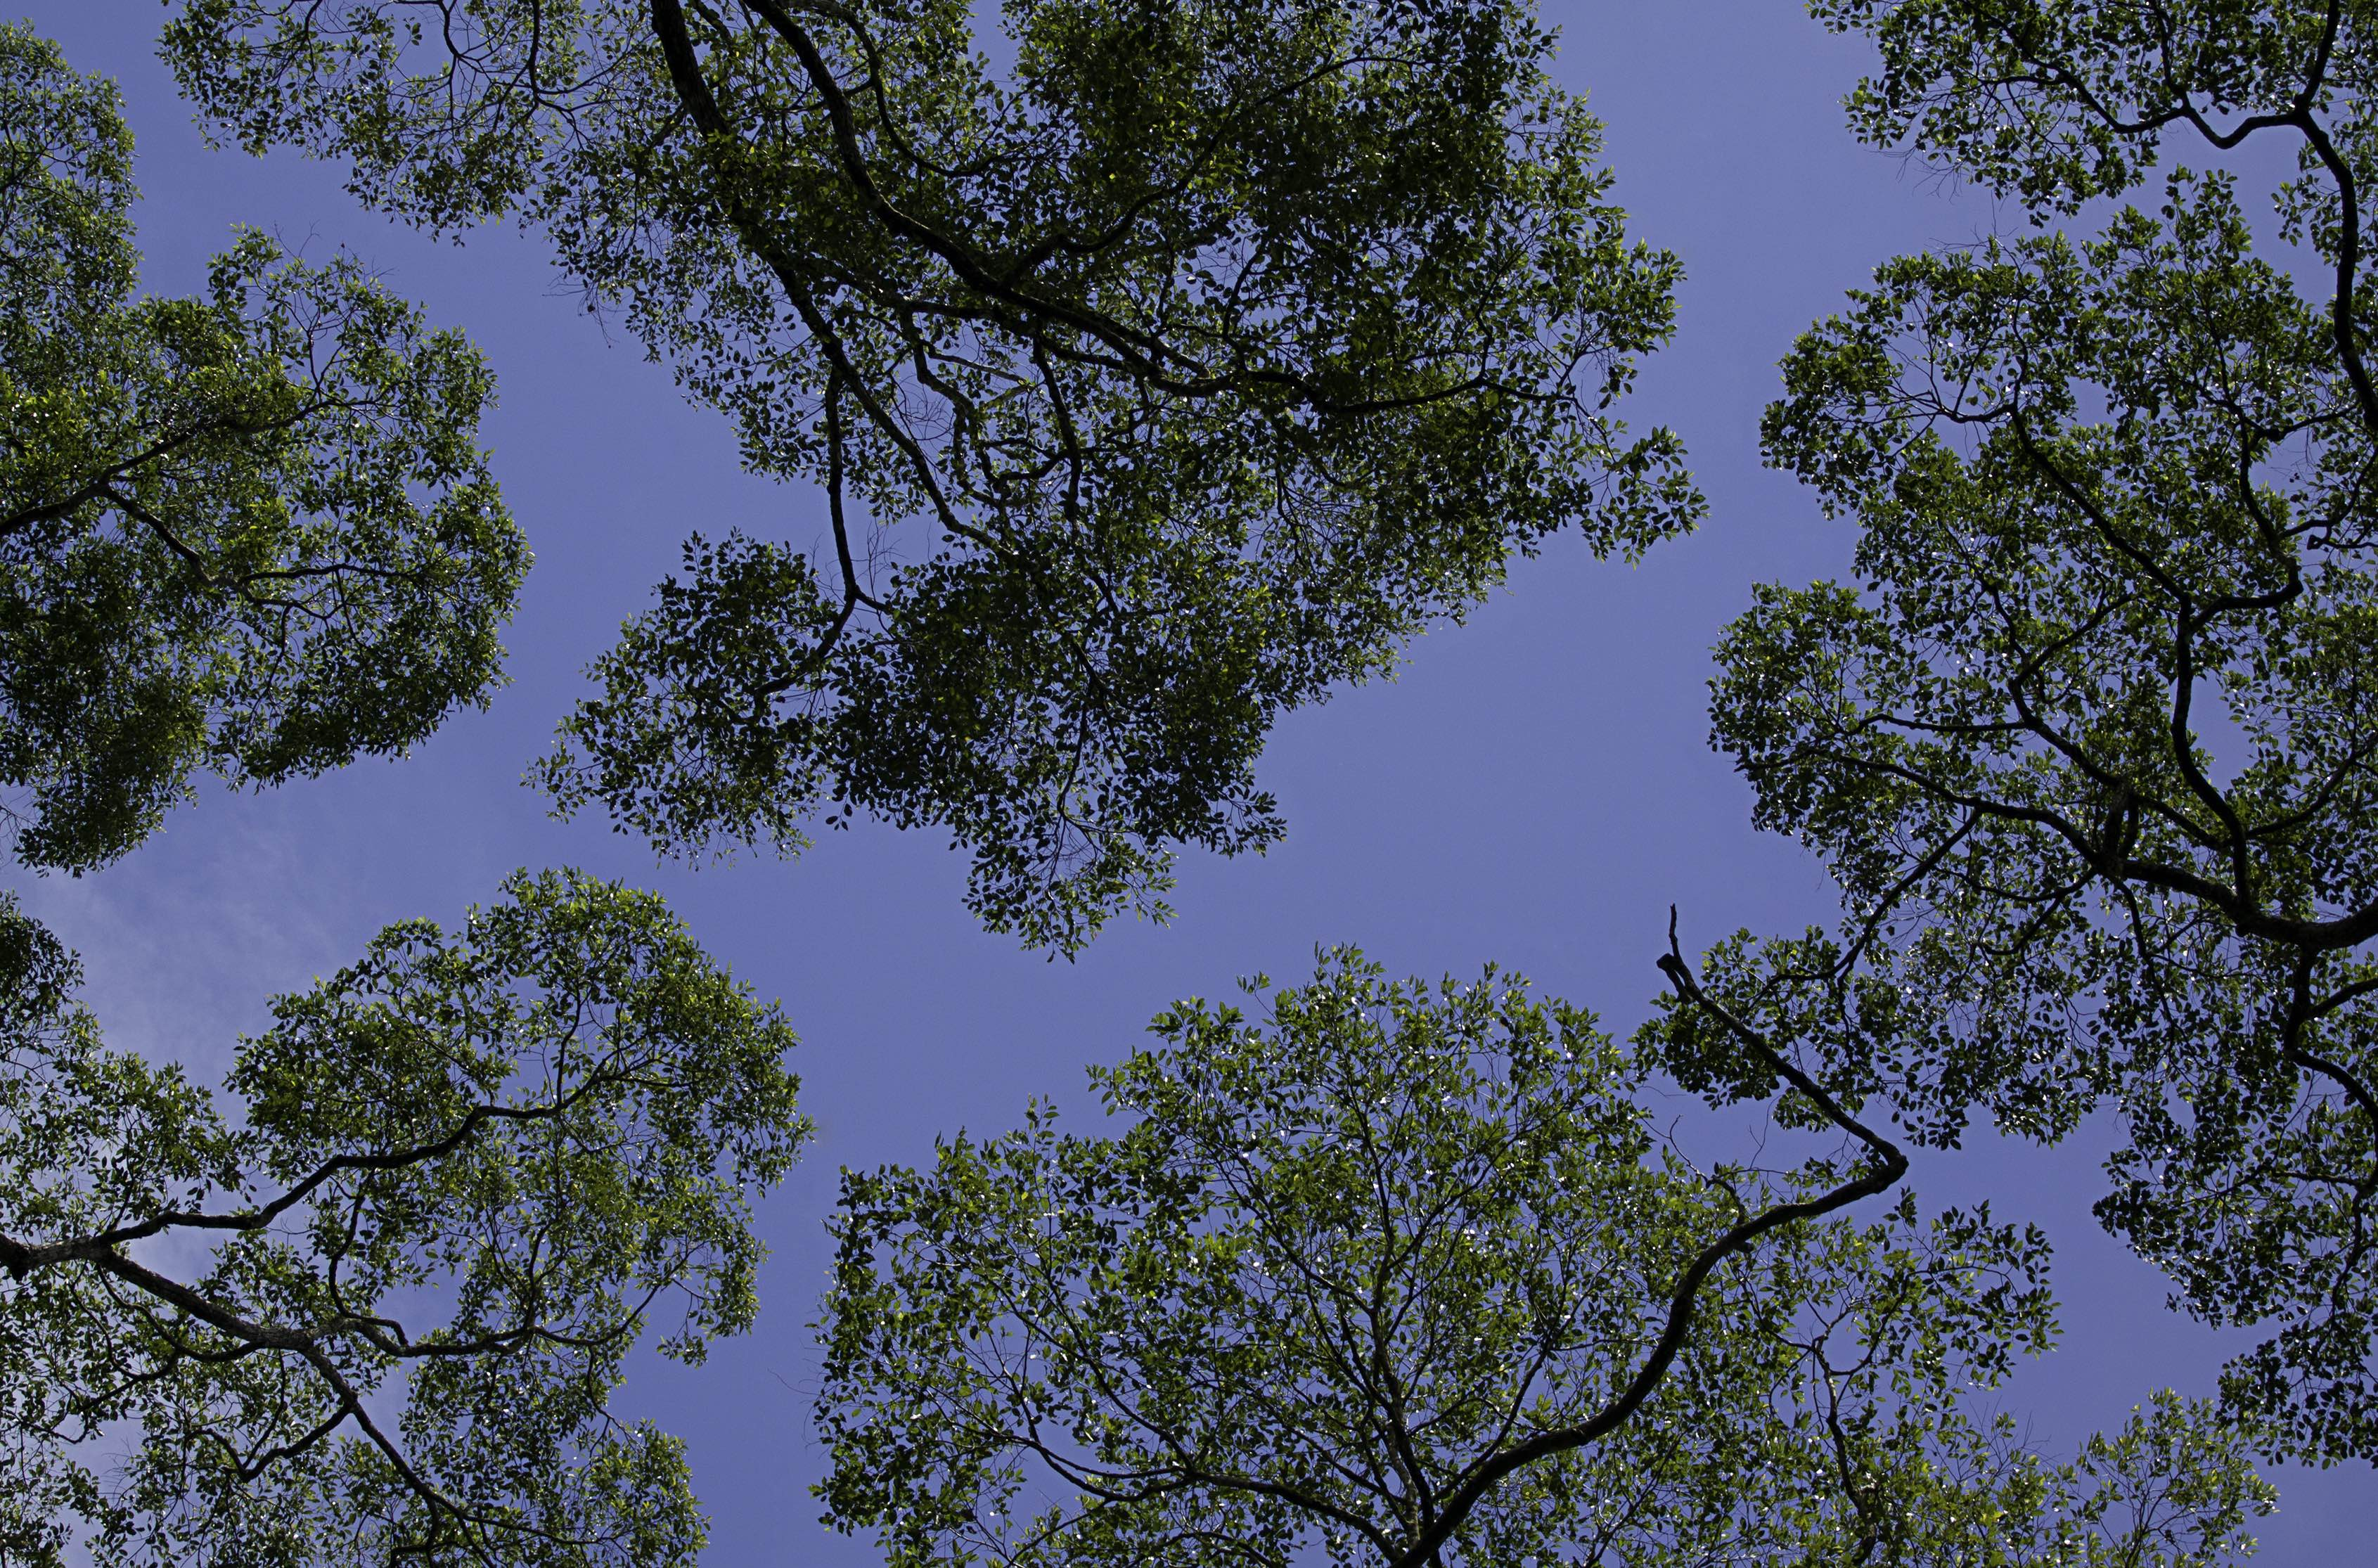
\includegraphics[width=0.6\linewidth]{dcp}
	\caption{Example of a digital cover photo taken with a regular camera lens \citep{dcp2010}.}
	\label{dcp}
\end{figure}

\section{Processing canopy photographs}

There are many software packages for processing and analysing forest canopy structure from hemispherical photographs, e.g. WinScanopy, CAN-EYE. I think processing with freely available, scriptable, open tools is more flexible, reproducible, and future-proof, and should be preferred for academic research. This part of the guide demonstrates a workflow for processing photos using Fiji \citep{Schindelin2012}, an open source software package built on top of ImageJ2 \citep{Rueden2017}, an image processing software popular among biologists. Much of the instruction in this guide will probably work with ImageJ, ImageJ2 and Fiji. Throughout the rest of the guide, when I refer to ImageJ I actually mean Fiji.

\subsection{Differentiating between plant and sky}

To calculate various metrics of forest canopy structure, it is necessary to partition the photo into areas of plant material and sky. A straightforward method for this relies on the assumption that the sky will be much brighter than the plant material. This is largely true for a correctly exposed photo. Note that in this process we are actually calculating PAI, rather than PAI. PAI includes non-leaf plant material such as wood, as it is difficult to separate leaves from branches using photographic techniques. Bear in mind then, that the PAI will be an over-estimate of the true LAI. The steps below describes how to partition an image based on pixel brightness, in ImageJ. This process returns an image with white pixels for sky and black pixels for plant material. Monospace blue font below refers to menu items in ImageJ to be selected.

\begin{enumerate}
	\item{Open ImageJ}
	\item{\menu{File $\rightarrow$ Open}, then select an image to process.}
	\item{\menu{Image $\rightarrow$ Type $\rightarrow$ 8-bit}. The image should become greyscale.}
	\item{\menu{Image $\rightarrow$ Adjust $\rightarrow$ Threshold}, and adjust the two sliders in the \menu{Threshold} window so all plant material is highlighted red and none of the sky is highlighted, or as near as you can get it. Click \menu{Apply} to binarize the image. The image should now be a mixture of black and white. The image should have black plant material and white sky.}
	\item{Save the newly binarized image as a \file{.tif}.}
\end{enumerate}

\begin{figure}[H]
\centering
	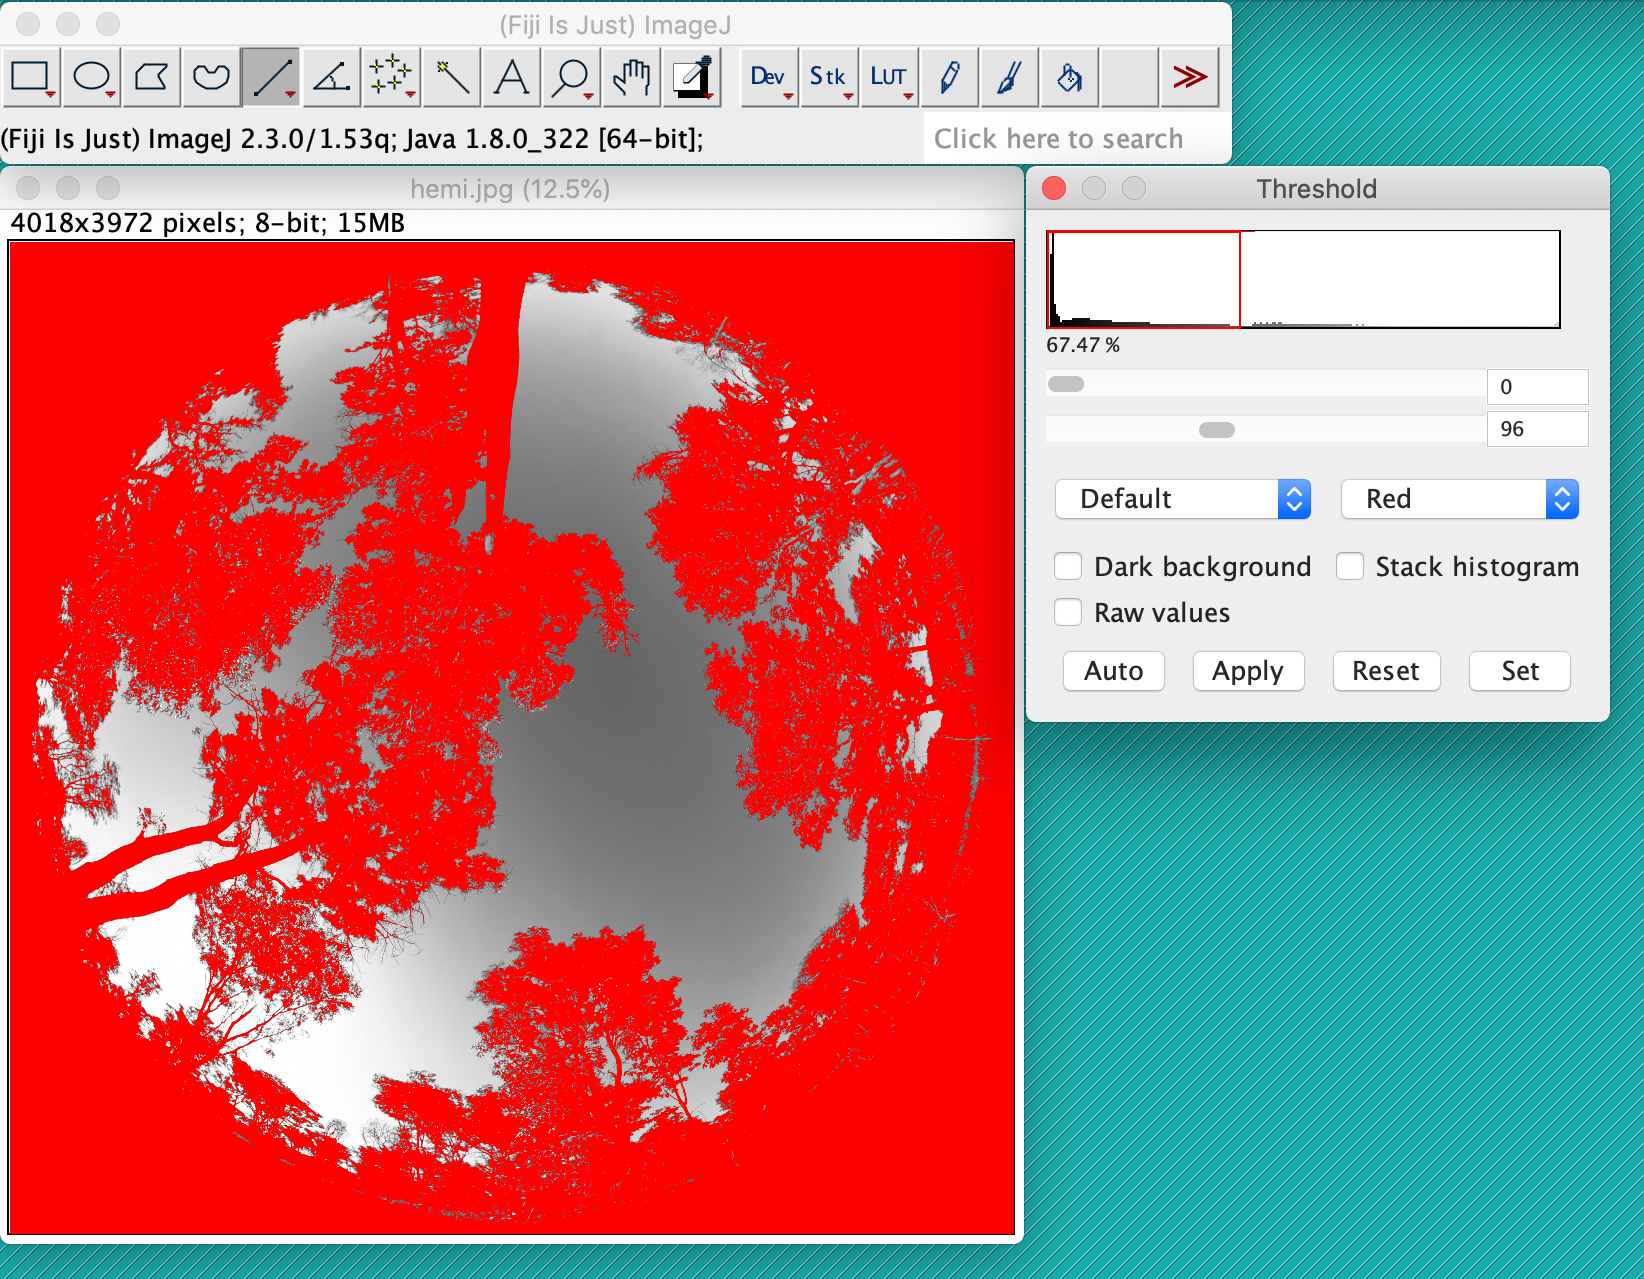
\includegraphics[width=0.8\textwidth]{threshold}
	\caption{Screenshot of the binarization process in ImageJ.}
	\label{threshold}
\end{figure}

The above process can be automated with an ImageJ macro (\autoref{binarize}), but this removes the ability to manually threshold each image, relying instead on one of a number of binarization algorithms provided in ImageJ. This technique should only be used when you are confident that all images are consistently exposed. 

Macros should be saved as a \file{.ijm} file and called within ImageJ with \menu{Plugins $\rightarrow$ Macros $\rightarrow$ Run..}. For a full list of macro functions available in ImageJ, consult the documentation (\url{https://imagej.nih.gov/ij/developer/macro/functions.html}). 

\begin{minipage}{\linewidth}
\lstinputlisting[label=binarize,caption=ImageJ macro to binarize all images in a nominated directory. The macro can also be found in \file{binarize.ijm}.]{src/binarize.ijm}
\end{minipage}

I find that the \texttt{Huang} \citep{Huang1995} binarization algorithm normally works well for thresholding canopy photos, but you should experiment with different algorithms to find the one which works best for your data. \texttt{Default} is also widely appropriate for canopy photos.

An alternative to simple thresholding of 8-bit greyscale images is to use a colour thresholding technique. Plant material often reflects very little blue, while the sky generally reflects much more, so one can threshold using only the blue channel of the image \citep{Brusa2014}. To binarize using a colour threshold:

\begin{enumerate}
	\item{Open ImageJ}
	\item{\menu{File $\rightarrow{}$ Open}, then select an image to process.}
	\item{\menu{Image $\rightarrow{}$ Adjust $\rightarrow{}$ Color Threshold...}}
	\item{\menu{Color space} = \numval{RGB}}
	\item{Adjust the sliders to highlight all the plant material}
	\item{\menu{Process $\rightarrow{}$ Binary $\rightarrow{}$ Convert to Mask}. The image should now have black plant material and white sky.}
\end{enumerate}

\begin{figure}[H]
	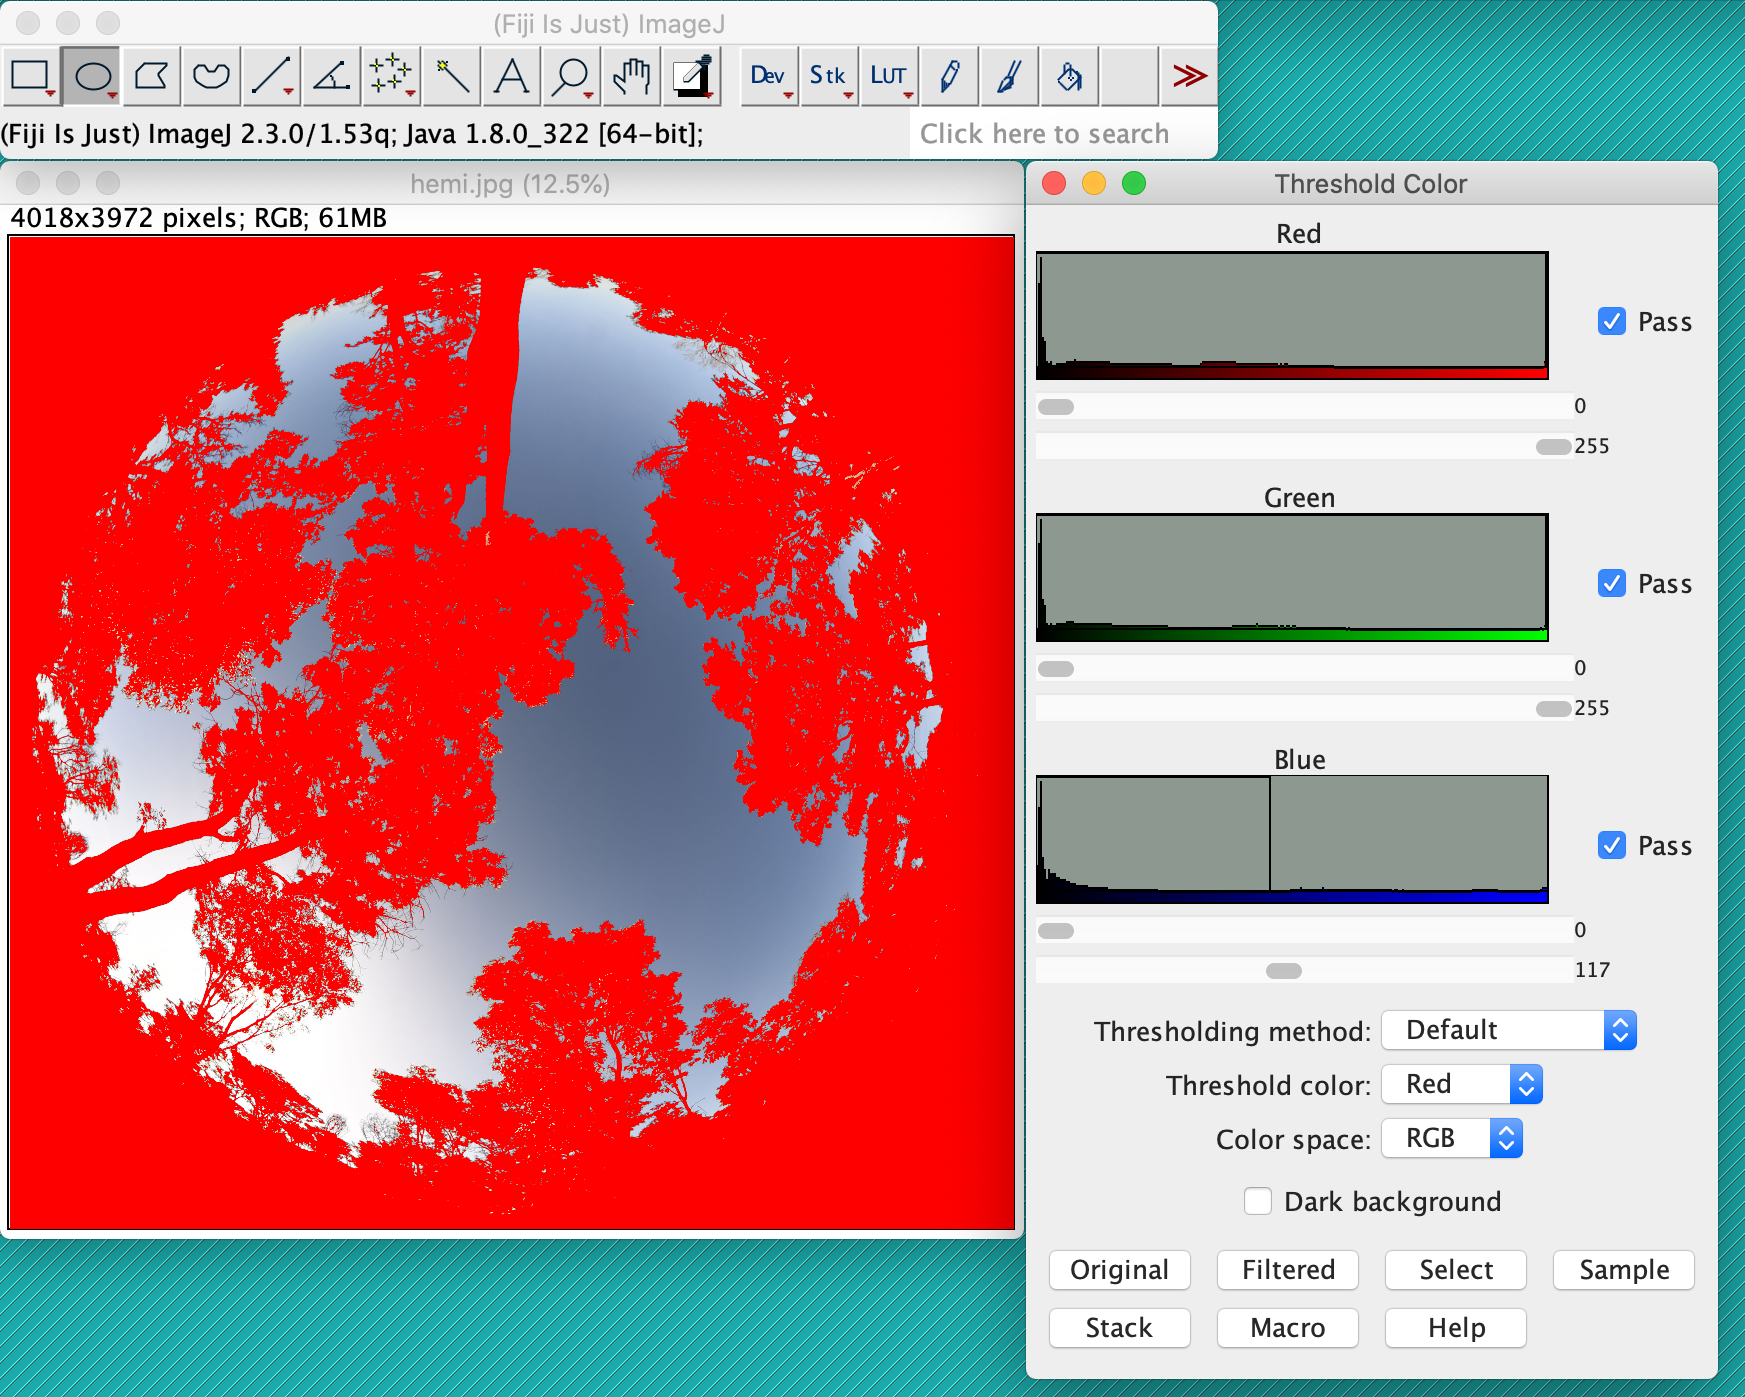
\includegraphics[width=0.8\linewidth]{colour_threshold}
	\caption{Screenshot of the color thresholding process in ImageJ.}
	\label{colour_threshold}
\end{figure}

\begin{minipage}{\linewidth}
\lstinputlisting[label=binarize_blue, caption=ImageJ macro to binarize images by the blue colour channel. The macro can also be found in \file{binarize\_blue.ijm}.]{src/binarize_blue.ijm}
\end{minipage}

\subsection{Cropping a circular image} \label{circle}

Sometimes, it's desirable to crop a hemispherical photo to a smaller circle with a known angle of view (zenith angle). A common convention is to crop an image to a 60\textdegree{} angular field of view. See \autoref{fov} for more information. Fisheye lenses have different projection functions which map the curved image onto a flat surface. Here is a list of common projection functions for different lenses:

\begin{itemize}
	\item{Equisolid (equal area) - $R = 2f\sin{(\theta/2)}$}
	\item{Equidistant - $R = f\theta$}
	\item{Orthographic - $R = f\sin{(\theta)}$}
	\item{Stereographic - $R = 2f\tan{(\theta/2)}$}
	\item{Thoby fisheye - $R = 1.47f\sin{(0.713\theta)}$}
\end{itemize}

\begin{figure}[H]
	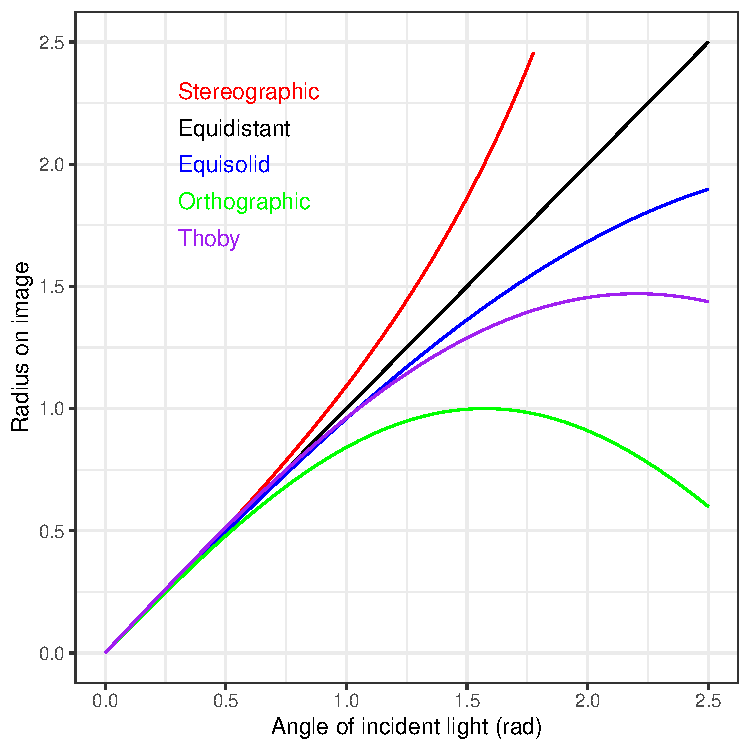
\includegraphics[width=0.75\textwidth]{lens_proj}
	\caption{Comparison of common fisheye lens projection functions.}
	\label{lens_proj}
\end{figure}

where $R$ is the radial position of a point on the image on the sensor, $f$ is the focal length of the lens, and $\theta$ is the angle in radians of incident light on the lens. Here is a diagram of what those values equate to on the camera lens.

\begin{figure}[H]
\centering
	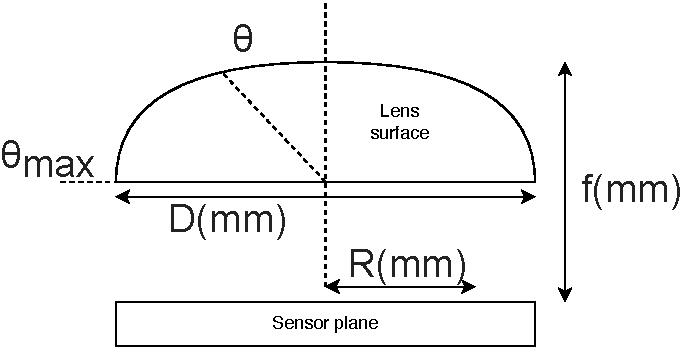
\includegraphics[width=\textwidth]{fov_diagram.drawio}
	\caption{Schematic diagram of a camera lens and sensor, demonstrating the measurements used when cropping an image to a given angular field of view.}
	\label{fov_diagram}
\end{figure}

The Sigma 8 mm lens in the ``ideal product list'' (\autoref{inform}) uses an equisolid projection. Equisolid lenses are preferred for hemispherical photography because they maintain an equal area for each pixel, i.e. a pixel projected through the lens has the same solid angle irrespective of the incident light angle. Below is a function written in the R programming language which calculates the radius of the circle in pixels for a desired angular field of view for the equisolid projection (\autoref{fov_func}).

\begin{minipage}{\linewidth}
\lstinputlisting[language=R, label=fov_func, firstline=14, lastline=28, caption=R function to calculate the pixel radius of a circle with a given zenith angle. Also found in \file{fov\_func.R}.]{src/fov_func.R}
\end{minipage}

The pixel pitch of the sensor is the real distance (in $\mu$m) from the centre of one pixel on the sensor to the centre of the next, in the case of the Sigma 8 mm it's 5.95 $\mu$m. This information can generally be found by querying the technical specifications for the camera, which may be available from the manufacturer or possibly found on online forums.

To crop an image to a given circular radius, I recommend using ImageMagick \citep{imagemagick}. You can download ImageMagick for your platform from \url{https://imagemagick.org/index.php}. \autoref{im_circle} can be saved as a shell script to crop multiple images to a circle of a particular radius.

\begin{minipage}{\linewidth}
\lstinputlisting[language=bash, label=im_circle, caption=Shell script to crop many images to a circle of a given radius. Provide the script with the circle radius in pixels as an integer and a list of files to be cropped. Also found in \file{im\_circle.sh}.]{src/im_circle.sh}
\end{minipage}


\subsection{Calculating gap fraction with ImageJ} \label{gapfrac}

The process for calculating gap fraction is fairly simple. Basically, from a  binarized image, you simply count the number of pixels in the image which are sky, i.e. white in the binarized image, then divide by the total number of pixels in the image. It's slightly more complicated when the image is a circle within a larger frame, but not much. The process for estimating canopy cover with DCP is identical to the process for estimating gap fraction from a hemispherical photograph. 

To calculate gap fraction: 

\begin{enumerate}
	\item{Open ImageJ}
	\item{\menu{File $\rightarrow$ Open} then select a binarized image.} 
	\item{\menu{Edit $\rightarrow$ Invert} to invert the colours, making the sky black and plant material white.}
	\item{\menu{Analyze $\rightarrow$ Analyze Particles...}}
		\begin{enumerate}
			\item{\menu{Size (pixel\textsuperscript{2})} = \numval{0-Infinity}}
			\item{\menu{Circularity} = \numval{0-1}}
			\item{\menu{Show} = \numval{Nothing}}
			\item{Check \menu{Summarize}}
		\end{enumerate}
	\item{The results should appear in a table, the gap fraction value is \menu{\%Area}.}
\end{enumerate}

\autoref{gap_frac_image} performs the same process but for a directory of images and exports a \file{.csv} spreadsheet file of the results. Remember to change the user inputs to point to where you would like images to be opened from and the spreadsheet saved to.

\begin{minipage}{\linewidth}
\lstinputlisting[label=gap_frac_image, caption=ImageJ macro to calculate the gap fraction of a full image. The macro can also be found in \file{gap\_frac\_image.ijm}.]{src/gap_frac_image.ijm}
\end{minipage}

The process is similar for a circular image, except a circle selection is created to exclude the black uninformative parts of the image before running \menu{Analyze Particles...}. See \autoref{gap_frac_circle} for the macro. 

\begin{figure}[H]
	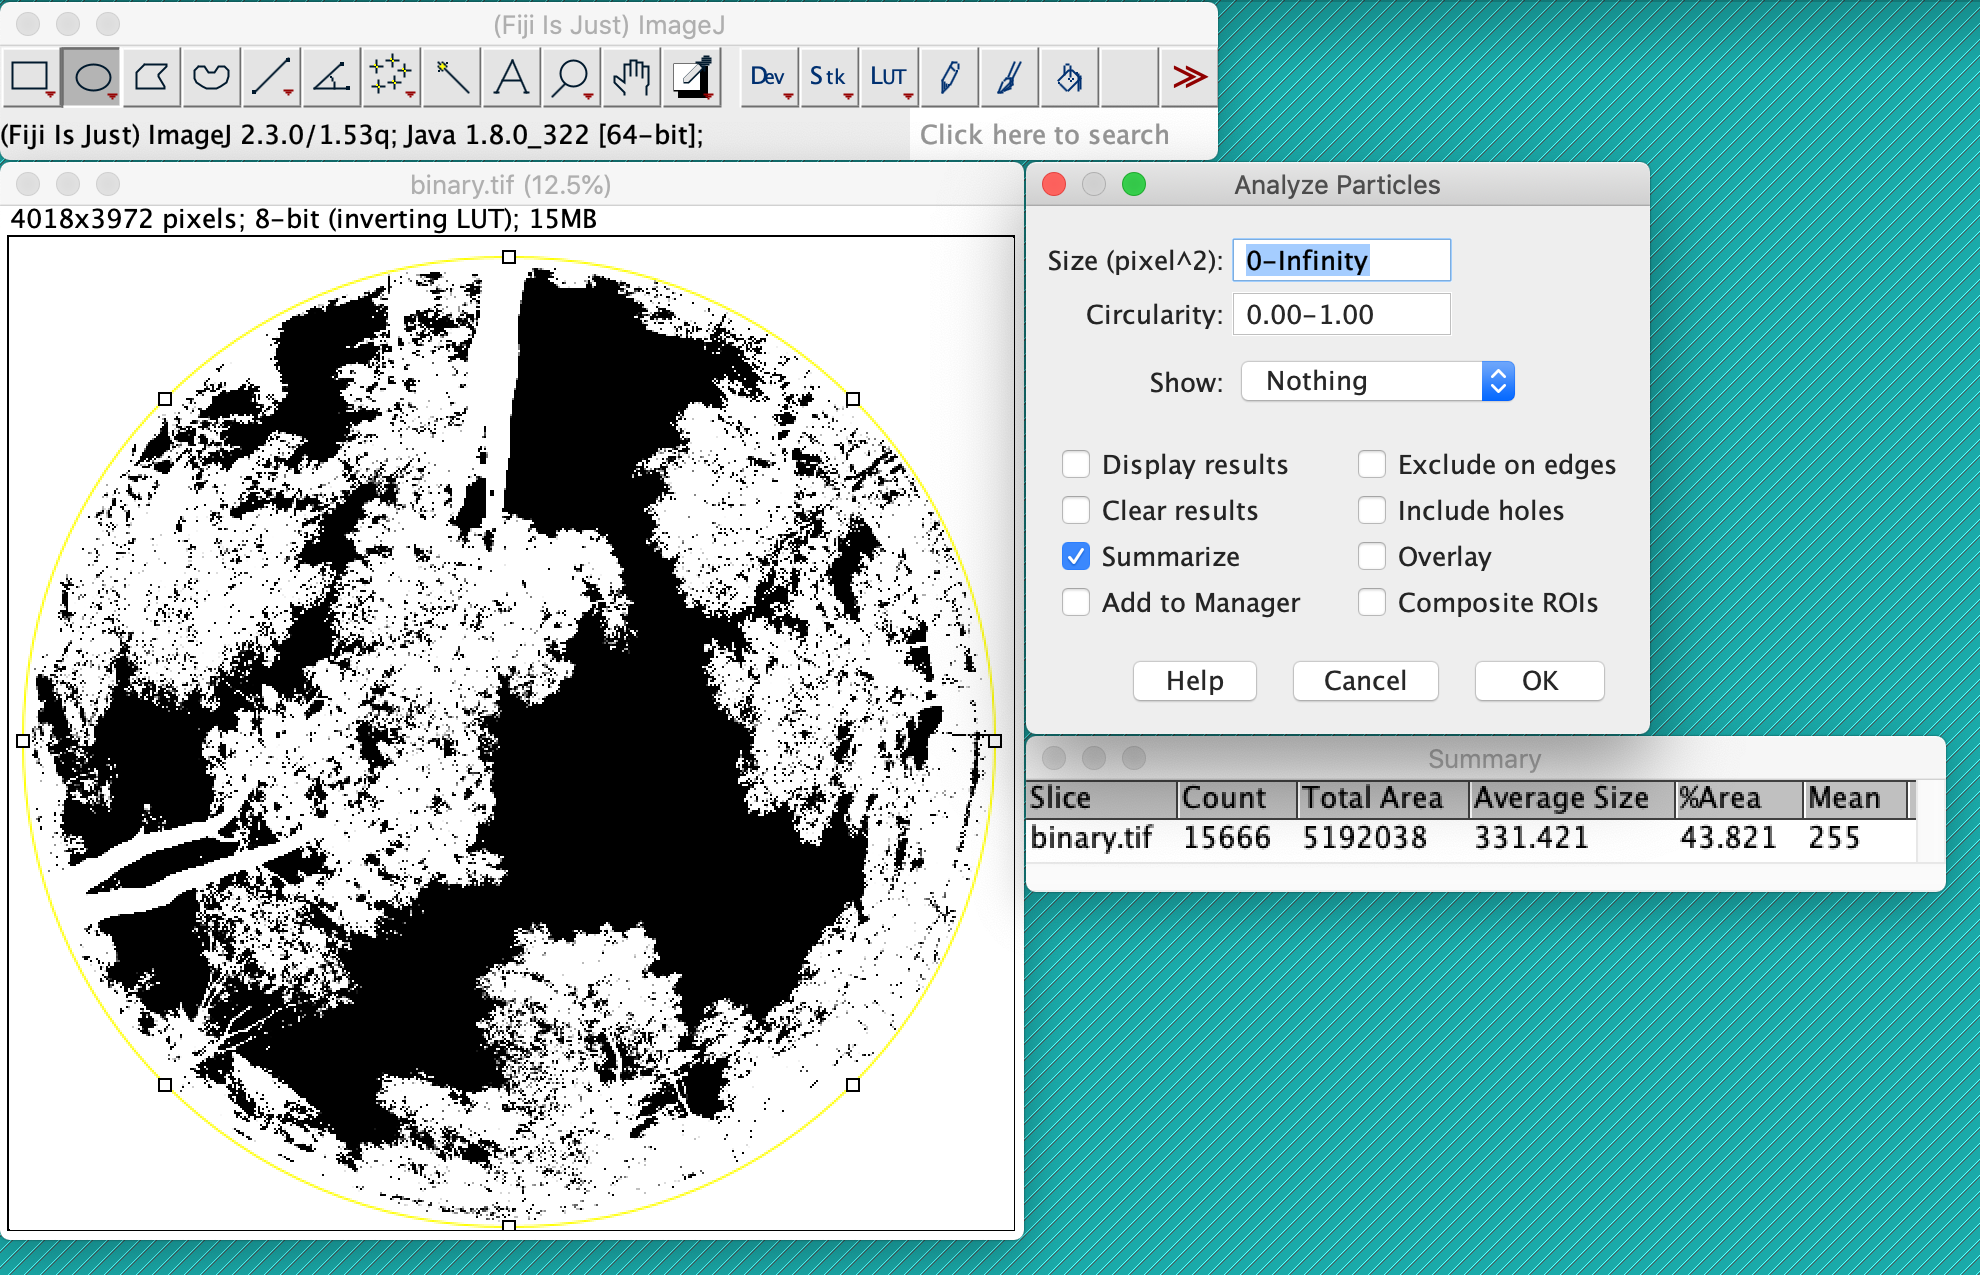
\includegraphics[width=0.8\linewidth]{particles}
	\caption{Screenshot of the particle analysis process for a circular image in ImageJ.}
	\label{particles}
\end{figure}

\begin{minipage}{\linewidth}
\lstinputlisting[label=gap_frac_circle, caption=ImageJ macro to calculate the gap fraction of a circular selection of an image. The macro can also be found in \file{gap\_frac\_circle.ijm}.]{src/gap_frac_circle.ijm}
\end{minipage}

The circular diameter of the image to fill \texttt{circle\_diam} can be measured in ImageJ by selecting \menu{Straight Line} from the toolbar then drawing a straight line across the centre of the circular image. Then select \menu{Analyze $\rightarrow$ Measure} to get the length of the line in the Results table.

\subsection{Calculating Leaf Area Index in R}

This part of the guide relies mostly on code written by Hans ter Steege in the HemiPhot R package \citep{Steege2018}, which ports WinPhot into the R language. WinPhot was originally written by Hans ter Steege in 1997 in Pascal, and Hemiphot can be seen as the natural progression of this software. Winphot is now obsolete and has been unmaintained since Windows XP. The code includes functions for thresholding and binarizing images, but I prefer to do this step in ImageJ because I have more control over how the images are thresholded this way. The snippets below describe a workflow for processing multiple binarized images in Hemiphot using R:

\vspace{0.5cm}
\begin{minipage}{\linewidth}
0. Preamble, load packages and functions.
\lstinputlisting[language=R, linerange=5-9]{src/hemiphot_example.R}
\end{minipage}

\begin{minipage}{\linewidth}
1. Read in all the previously thresholded and binarized \file{.tif} images and create an empty data frame which will later be filled with canopy structure metrics like LAI and canopy openness.
\lstinputlisting[language=R, linerange=11-22]{src/hemiphot_example.R}
\end{minipage}


\begin{minipage}{\linewidth}
	2. Set some parameters for the day of year and the location the photos are being taken. Approximate location (0.1\textdegree{} latitude) is good enough. Note that the values below are for somewhere in Africa and should be changed:
\lstinputlisting[language=R, linerange=24-28]{src/hemiphot_example.R}
\end{minipage}


\begin{minipage}{\linewidth}
3. Set some parameters for the images, cropping them to a circle and setting the threshold. Even if the images have been thresholded already, thresholding them again won't change anything. These parameters are for the equipment listed in the ``ideal product list'', so may need to be changed depending on your equipment:
\lstinputlisting[language=R, linerange=30-33]{src/hemiphot_example.R}
\end{minipage}


\begin{minipage}{\linewidth}
4. Set some atmospheric parameters. The metrics affected by these parameters are: \texttt{DirectAbove}, \texttt{DiffAbove}, \texttt{DirectBelow} and \texttt{DiffBelow}. If these metrics are of no interest to you, just fill these parameters with random decimals between zero and one.
\lstinputlisting[language=R, linerange=35-39]{src/hemiphot_example.R}
\end{minipage}


\begin{minipage}{\linewidth}
5. Run a \texttt{for} loop to calculate metrics for each image.
\lstinputlisting[language=R, linerange=41-68]{src/hemiphot_example.R}
\end{minipage}

6. Finally, look at the output, which is stored in \texttt{out}.

There are many other functions in the source code for Hemiphot. It is recommended to read through them along with the documentation to see what is appropriate for your needs. A copy of the script above is included in \file{hemiphot\_example.R}.

\subsection{Zenith angle for LAI calculations} \label{fov}

This is the only reference I have found in the literature which discusses why the angle of view should be limited from a full 90\textdegree{} hemispherical image. It can be supposed that below 60\textdegree{}, in most forest canopies, variation in tree canopy density does little to affect sunlight penetration, due to the greater depth of canopy at these angles. Additionally, for many fisheye lenses, angles below 60\textdegree{} introduce significant visual artefacts and distortion, which may lead to biased results. 

\begin{minipage}{\linewidth}
\begin{framed}
In the range from zero to about 60 zenith angle the canopy effects are more significant. This is the useful working range of most hemispherical photograph data.

-- \citet{Jupp2009}
\end{framed}
\end{minipage}


\section{Alternatives to photography}

Some devices measure light intensity to estimate LAI. The AccuPAR LP-80 Ceptometer \citep{accupar2013} has a long ``wand'' with many PAR (Photosynthetically Active Radiation) sensors along its length, which are used in conjunction with an external PAR sensor designed to be held outside the canopy as a reference value, to estimate LAI using equations which take into account direct incident light, and light scattered by canopy material \citep{Goudriaan1988}. The LiCOR LAI-2000 \citep{lai2000, Cutini1998} uses a fisheye light sensor to measure diffuse radiation in five concentric rings. As with the LP-80, a reference value above the canopy is also taken so that gap fraction can be estimated as the ratio between the above and below canopy gap fraction readings. 

Terrestrial or airborne Light-Detection And Ranging (LiDAR) equipment can be used to estimate canopy cover and the vertical distribution of canopy material. Equipment is expensive and processing is complex, but this method is currently the most precise and accurate \citep{Seidel2011} way to measure gap fraction, canopy cover, and LAI, as it uses an active radiation source, rather than the sun, to detect canopy gaps. 

Periscope densitometers are a simple way to estimate canopy cover across an area (\autoref{periscope_densitometer}). A simple periscope tube with a mirror is marked with a cross. The periscope is pointed upwards and the operator records the presence or absence of plant material in the centre of the cross. A dense grid of measurements is recorded which can then be converted to a percentage canopy cover \citep{GRS}. As the data is binary, it is very straightforward to estimate the uncertainty of the canopy cover estimate given the density of points across the area. If you are only interested in canopy cover and not in LAI or gap fraction, a periscope densitometer is a good method, as is digital cover photography.

\begin{figure}[H]
	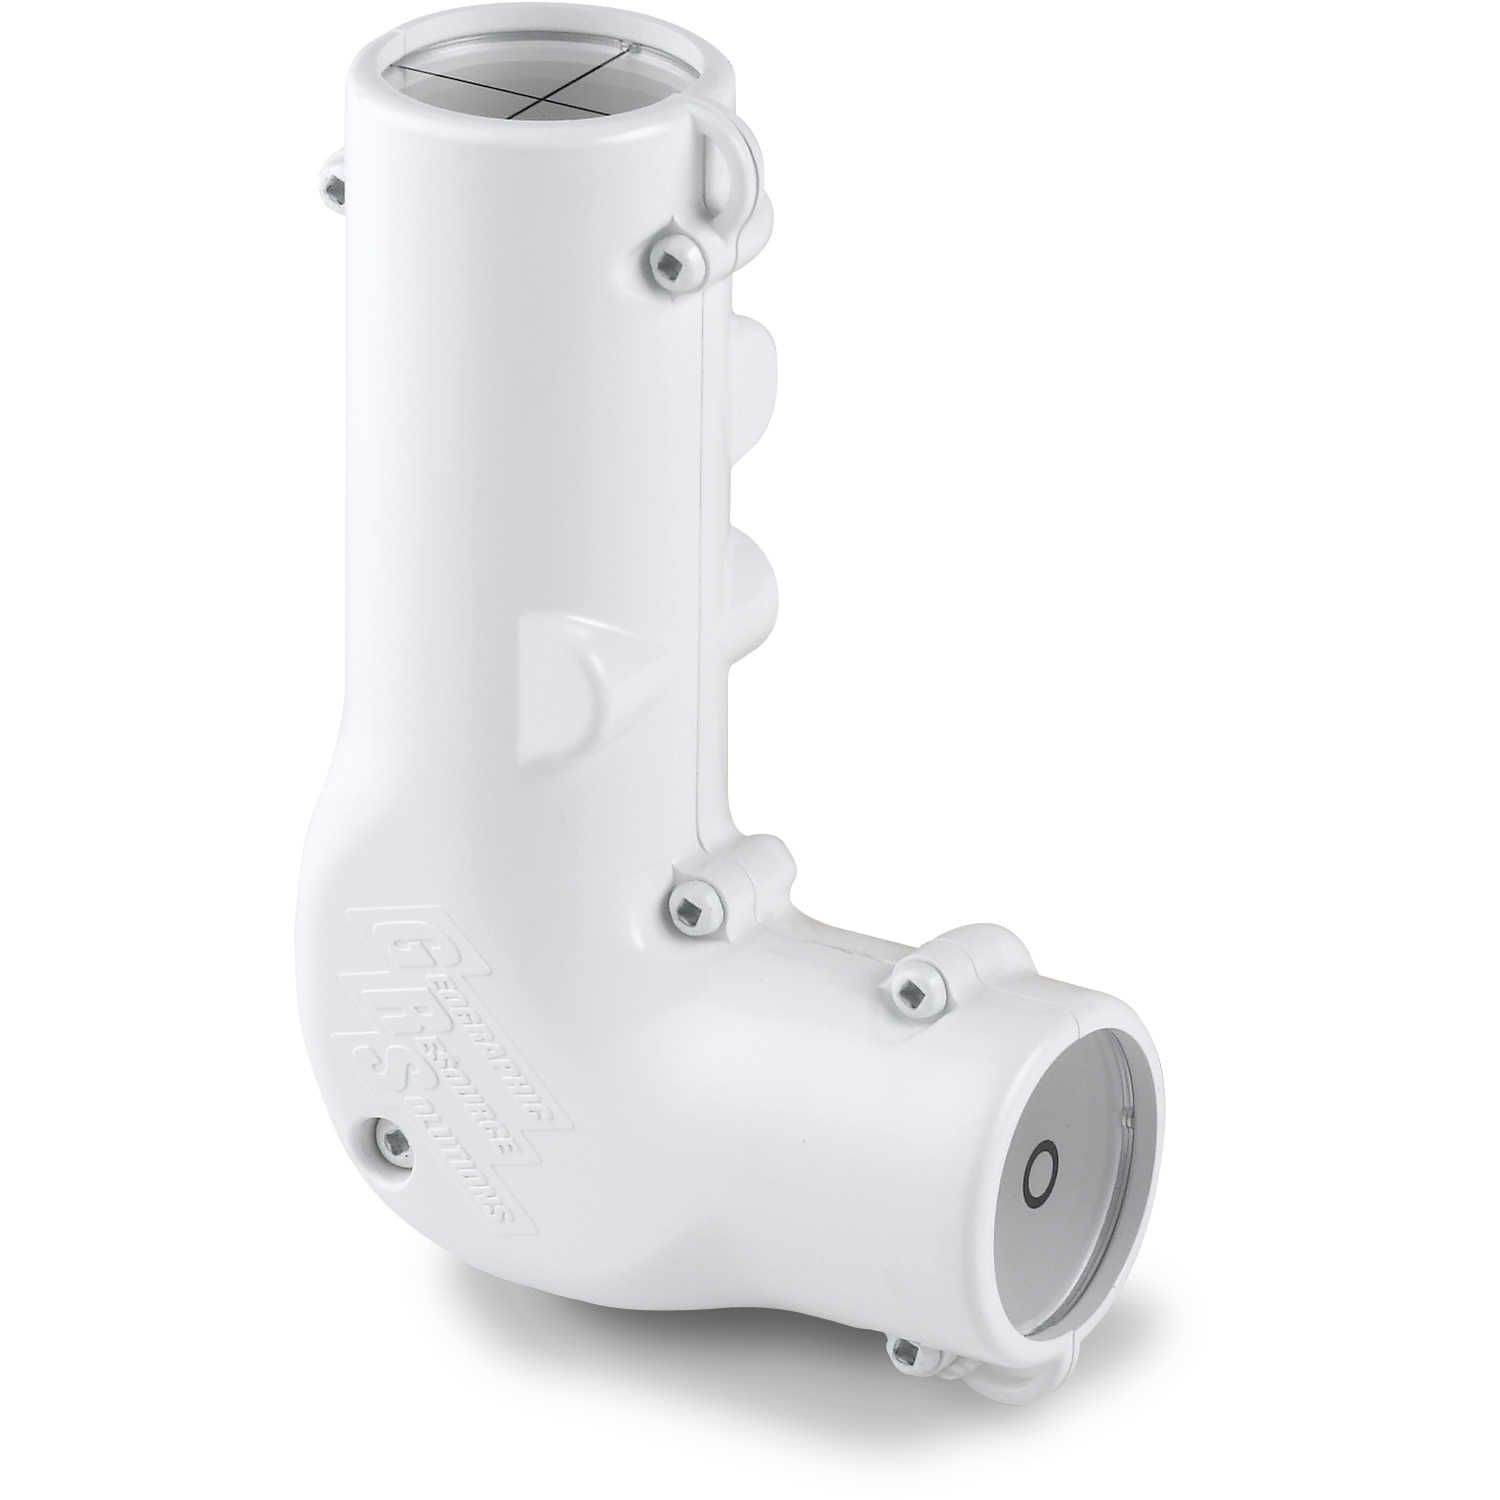
\includegraphics[width=0.5\linewidth]{periscope_densitometer}
	\caption{A periscope densitometer, manufactured by \citet{GRS}.}
	\label{periscope_densitometer}
\end{figure}

Reflective dish densitometers used to be the industry standard in forestry for estimating gap fraction (\autoref{disco_densitometer}). A convex mirror surface is divided into a grid to facilitate the estimation of the percentage of sky covered by plant material \citep{Lemmon1956}. This method, while previously commonplace in ecology and forestry, is now not recommended, as it has been shown that large recording biases can occur, even when measurements are taken by a trained operator \citep{Korhonen2006}.

\begin{figure}[H]
	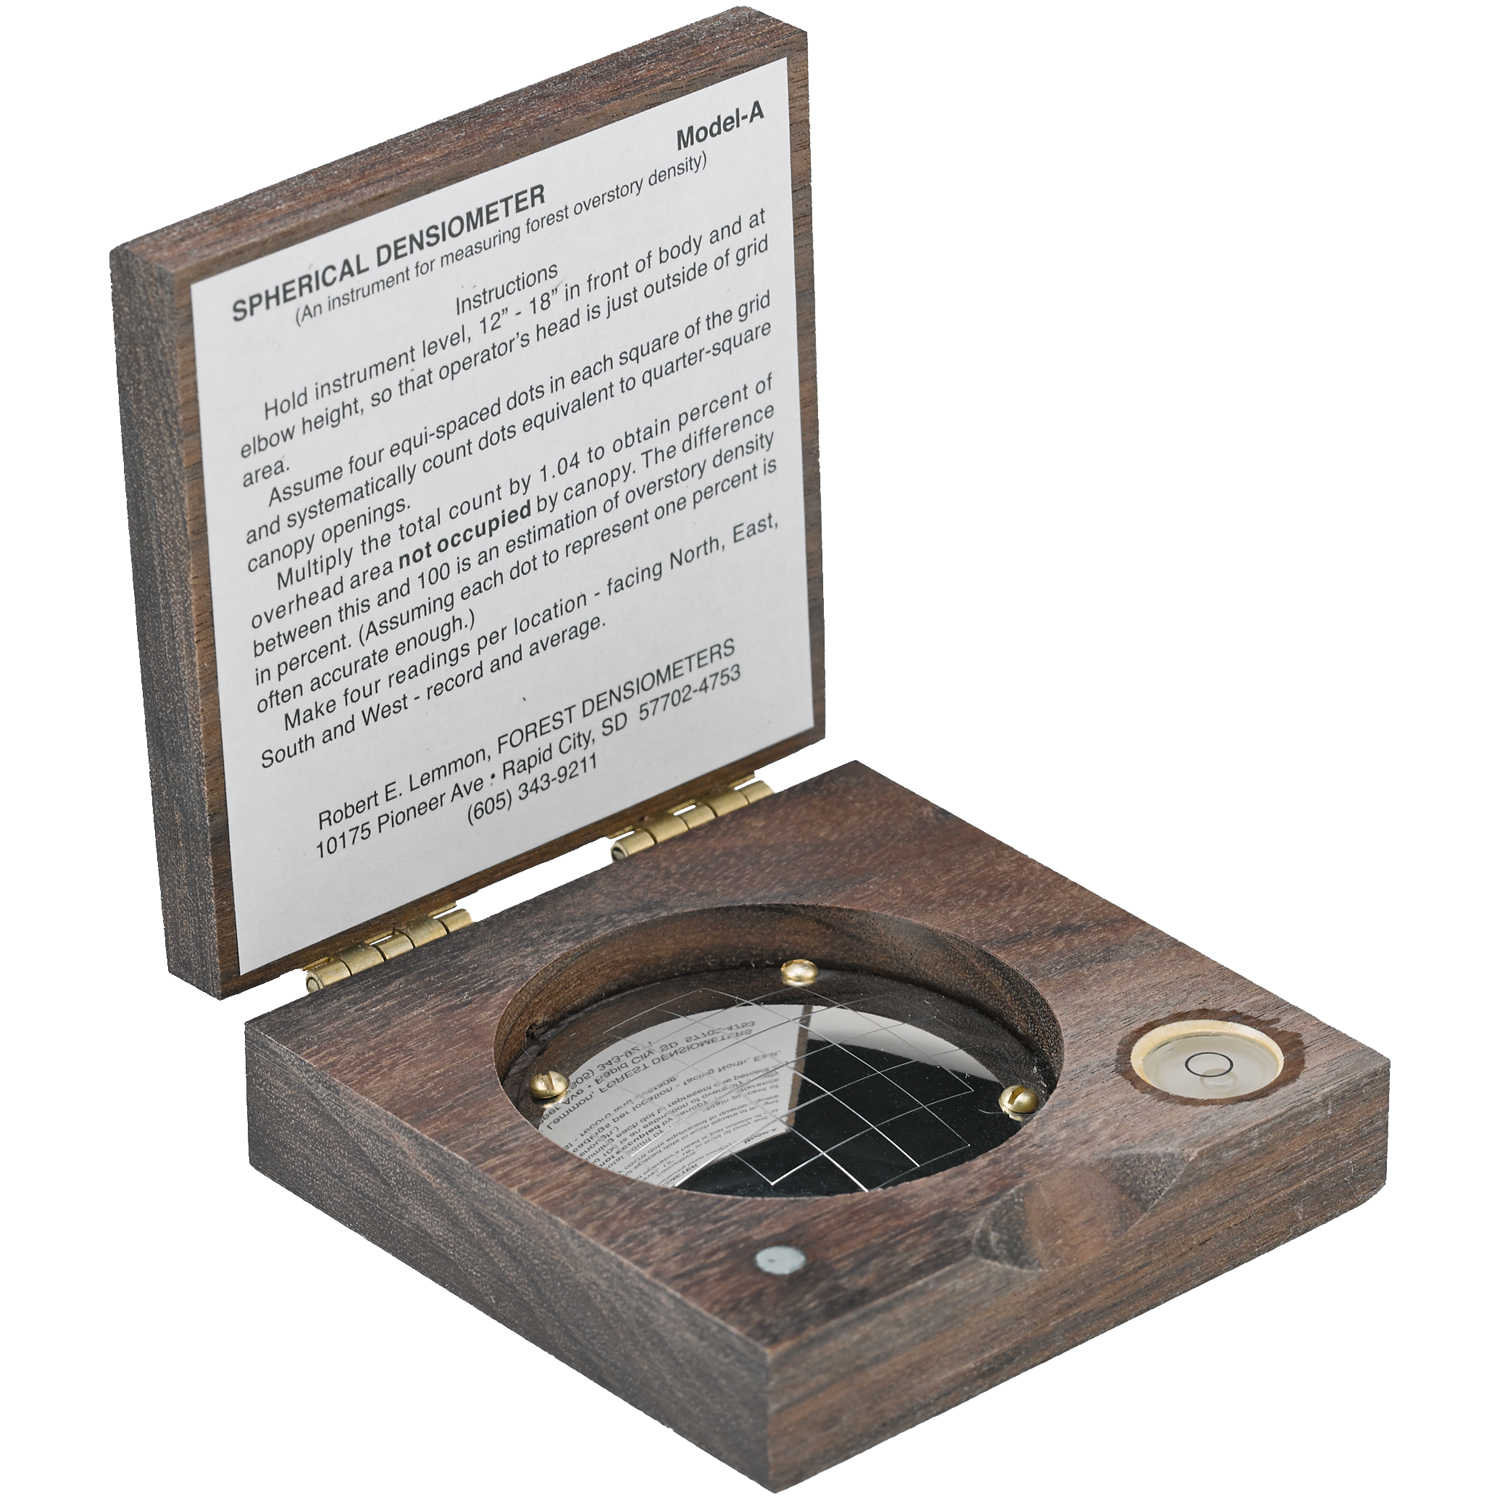
\includegraphics[width=0.5\linewidth]{disco_densitometer}
	\caption{A reflective dish densitometer, affectionately referred to as a ``disco ball''.}
	\label{disco_densitometer}
\end{figure}

In a deciduous forest canopy with clear seasonal leaf growth and senescence, it is possible to estimate LAI simply by collecting leaves after they fall from the tree. A leaf trap of known dimensions is left on the forest floor for a known period of time to capture falling leaves. The area of these individual leaves is measured to estimate the total leaf area of the canopy. This method has an advantage over many indirect methods in that it can easily separate woody material from leaf material to give the true LAI, rather than the Plant Area Index (PAI). 

Direct leaf harvesting can be conducted by removing branches within a known area of canopy and stripping the leaves. The area of the individual leaves is then measured to directly measure the total leaf area of the canopy. This method is destructive and laborious, and so is rarely used, but does provide the most accurate measure of LAI.

\printbibliography

\end{document}
